\documentclass[a4paper]{article}

%maximum figure number
\setcounter{totalnumber}{5}

%plus minus
\newcommand{\mypm}{\mathbin{\smash{%
\raisebox{0.35ex}{%
            $\underset{\raisebox{0.5ex}{$\smash -$}}{\smash+}$%
            }%
        }%
    }%
}

%diagbox
\usepackage{diagbox}

%figure inside text
\usepackage{wrapfig}

%layout config
\usepackage{calc}
\setlength\textwidth{7in}
\setlength\textheight{10in}
\setlength\oddsidemargin{(\paperwidth-\textwidth)/2 - 1in}
\setlength\topmargin{(\paperheight-\textheight
-\headheight-\headsep-\footskip)/2 - 1in}

%sinuit
\usepackage{siunitx}
%image insertion
\usepackage{graphicx} %image settings
\DeclareGraphicsExtensions{.pdf,.png,.jpg}

%math
\usepackage{amsmath} %math
%\usepackage{cmbright} %math font

%font
\usepackage{kotex}
\usepackage{fontspec}
\ifx가가
\setmainhangulfont[Ligatures=TeX,
BoldFont={KoPubBatang Medium}]{KoPubBatang Light}
\setsanshangulfont[Ligatures=TeX,
BoldFont={KoPubDotum Medium}]{KoPubDotum Light}
\setmainhanjafont[Ligatures=TeX,
BoldFont={KoPubBatang Medium}]{KoPubBatang Light}
\setsanshanjafont[Ligatures=TeX,
BoldFont={KoPubDotum Medium}]{KoPubDotum Light}
\xetexkofontregime[puncts=prevfont, colons=prevfont, cjksymbols=hangul]{latin}
\fi

%줄간격
\usepackage{setspace}
%\usepackage{indentfirst}
\setstretch{1.2}
\everydisplay{\setstretch{1.2}}

%subfloat
\usepackage{subfig}
% and
\newcommand{\shitn}{&}

\pagestyle{plain}
\title{물리 실험보고서 1}
\author{이한빈, 의예과 2016-13347}

\begin{document}


\numberwithin{equation}{section}
\maketitle

\section{Introduction}
 	Wheatstone Bridge은 4개의 저항과 검류계가 연결된 장치로서 미지의 저항을 측정하기 위해 사용된다.
 	\begin{figure}[h]
 		\centering
 		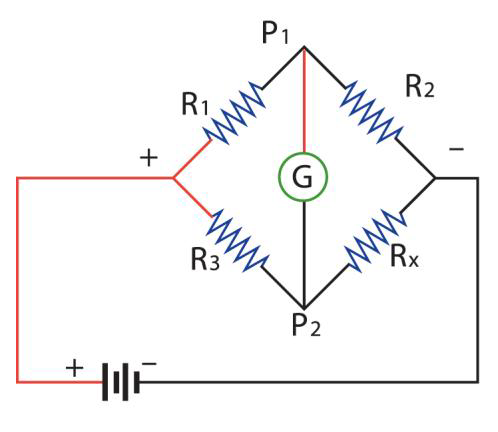
\includegraphics[width=0.2\textwidth]{img/wheatstone-bridge.png}
 		\caption{Wheatstone Bridge의 모식도} \label{fig:wheatstone}
 	\end{figure}

 	가변저항 $R_{x}$를 조절을 조절하면 검류계에 흐르는 전류가 0이 되도록 할 수 있는데 이 떄의 조건을 통해 미지 저항 $R_3$를 구할 수 있다.
 	$P_{1}P_{2}$사이에 전류가 흐르지 않는다는 것은 두 점 사이의 전위차가 0이라는 뜻이므로 $R_1$과 $R_2$에서의 전압강하 비율이 $R_3$과 $R_x$에서의 전압강하 비율과 같다는 뜻이다.
 	따라서 다음이 성립한다.
 	\begin{equation}
 		R_1:R_2 = R_3:R_x
 	\end{equation}
 	이를 변형하면 다음을 얻는다.

 	\begin{equation}
 		R_3 = \frac{R_1}{R_2}R_x
 		\label{eq:eq}
 	\end{equation}
 	이로부터 $R_1$과 $R_2$의 비율 $\frac{R_1}{R_2}$과 가변저항 $R_x$의 값을 알고 있으면 미지저항 $R_3$의 값을 알아낼 수 있다.

 	본 실험에서는 습동저항선을 통해 가변저항 $R_x$를 구현한다.
 	\begin{figure}[h]
 		\centering
 		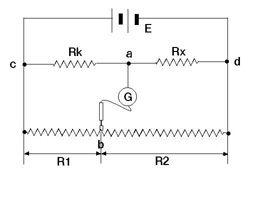
\includegraphics[width=0.25\textwidth]{img/line.jpg }
 		\caption{습동저항선} \label{fig:line}
 	\end{figure}

 	그림(\ref{fig:line})에서 볼 수 있듯이 점 b의 위치를 변화시키면 $R_1$과 $R_2$의 값이 바뀌므로 $\frac{R_1}{R_2}$의 값을 조절할 수 있다.
 	습동저항선의 두께와 비저항이 일정하므로 $R = \rho \frac{l}{A}$를 이용하면 $\frac{R_1}{R_2} = \frac{l_1}{l_2}$임을 알 수 있다. 
 	따라서 두 저항선의 길이를 측정하면 미지저항을 측정할 수 있다.

 	이 실험을 통해서 휘트스톤 브릿지를 이용하여 미지저항을 측정하고 이를 바탕으로 휘트스톤브릿지의 작동원리에 대해서 이해한다.

\newpage

 	\section{Method}
 	준비물: Ready-Set Wheatstone 실험장치 (5V 직류전원장치, 기지저항 100\si{\ohm}, 1\si{k\ohm}, 10\si{k\ohm}, 50\si{k\ohm}, 100\si{k\ohm}), 수백\si{\ohm}에서 수십\si{k\ohm}의 저항 12개, 1\si{\micro{}A} 디지털 검류계, 습동저항선 20\si{cm}, 측정용 버니어캘리퍼스), 전압계

 	\subsection{Wheatstone Bridge를 이용한 미지 저항 측정}
 	1) Ready-Set Wheatstone Bridge를 전원에 연결한다. \\
 	2) $R_x$의 다이얼을 돌려 미지저항 1을 택하고 스위치를 켠다. \\
 	3) $R_k$의 저항을 조절하여 검류계 값이 0을 가리킬 떄의 습동저항선 가리키게가 중앙에 최대한 가깝게 설정한다. \\
 	4) 이 때의 값을 버니어캘리퍼스를 통해 읽는다. \\
 	5) \ref{eq:eq}로부터 미지저항 $R_x$값을 측정한 후 기재한다. \\
 	6) $R_k$의 다이얼을 돌려 미지저항을 바꾸어가며 위의 과정을 2번에서 12번까지 반복한다. \\
 	*실제 실험에서는 3)의 전류 0 맞추는 과정을 실패한 경우가 있었다.
 	이럴 경우에는 전류 값을 최대한 0에 가깝게 하려고 했다. 

 	\subsection{전압계를 이용한 미지 저항 측정}
 	1) 전압계를 $R_x$사이에 고정시킨다. \\
 	2) $R_k$의 값을 1\si{k\ohm}에 고정시킨 후 전압계의 전압을 측정한다. \\
 	3) $R_x$의 값을 2~12로 바꾸어가며 위 과정을 반복한다.

\newpage

 	\section{Result}
 		\subsection{실험 장치들 스펙}
 		습동구리선의 전체길이 : 20\si{cm},
 		버니어캘리퍼스의 유효숫자 : 5개, 
 		회로에 인가된 총 전압 : 5\si{V}

 		\subsection{Wheatstone Bridge를 이용한 미지 저항 측정}
 	\begin{figure}[h]
 		\centering
 		\subfloat[미지저항에 따른 습동저항선 가리키게의 위치]{
 		\begin{tabular}[b]{|c|c|c|c|c|}
 		\hline 
 		전류(\si{\micro A}) & 거리(\si{cm}) & $R_k$(k\si{\ohm}) & $R_x$(번호) & $R_x$(\si{k\ohm})\\
 		\hline
 		0 & 13.32 & 1 & 1 \shitn 0.501\\
 		\hline
 		-8 & 18.05 & 1 & 2 \shitn 0.108\\
 		\hline
 		0 \shitn 6.70 \shitn 1 \shitn 3 \shitn 1.985 \\
 		\hline 
 		0 \shitn 12.71 \shitn 5 \shitn 4  \shitn 2.867\\
 		\hline
 		0 \shitn 7.97 \shitn 1 \shitn 5 \shitn 1.509 \\
 		\hline
 		0 \shitn 9.21 \shitn 5 \shitn 6  \shitn 5.857\\
 		\hline
 		5 \shitn 17.7 \shitn 1 \shitn 7 \shitn 0.129\\
 		\hline
 		8 \shitn 16.465 \shitn 1 \shitn 8 \shitn 0.214\\
 		\hline
 		-2 \shitn 15.85 \shitn 5 \shitn 9 \shitn 1.309\\
 		\hline
 		1 \shitn 11.67 \shitn 10 \shitn 10 \shitn 7.137\\
 		\hline
 		1 \shitn 15.09 \shitn 5 \shitn 11 \shitn 1.626\\
 		\hline
 		=3 \shitn 12.095 \shitn 1 \shitn 12 \shitn 0.653\\
 		\hline
 		\end{tabular}
 		\label{fig:result1}
 		}
 		\subfloat[표의 결과를 바탕으로 계산된 저항]{
 		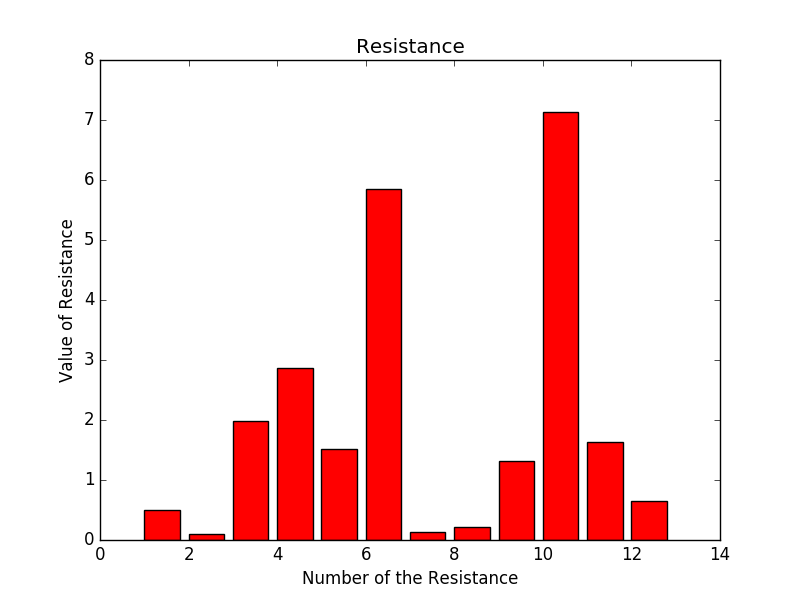
\includegraphics[width=0.4\textwidth]{img/figure1.png}
 		}
 	\end{figure}
 	저항은 $R_x = \frac{20-l}{l} R_k$로 계산되었다.


 	\subsection{전압계를 이용한 미지 저항 측정}
 	\begin{figure}[h]
 		\centering
 		\subfloat[미지 저항에 따른 $R_x$에 걸리는 전압]{
 		\begin{tabular}[b]{|c|c|c|c|}
 		\hline 
 		전압(\si{V}) & $R_k$(k\si{\ohm}) & $R_x$(번호) & $R_x$(\si{k\ohm})\\
 		\hline
 		2.8 & 1 & 1 & 1.272\\
 		\hline
 		1.5 & 1 & 2 & 0.428\\
 		\hline
 		3.45 \shitn 1 \shitn 3 \shitn 2.225\\
 		\hline 
 		4 \shitn 1 \shitn 4 \shitn 4.000 \\
 		\hline
 		3.35 \shitn 1 \shitn 5 \shitn 2.030 \\
 		\hline
 		4.1 \shitn 1 \shitn 6 \shitn 4.555\\
 		\hline
 		1.7 \shitn 1 \shitn 7 \shitn 0.515 \\
 		\hline
 		2.1 \shitn 1 \shitn 8 \shitn 0.724 \\
 		\hline
 		3.75 \shitn 1 \shitn 9 \shitn 3.000 \\
 		\hline
 		4.2 \shitn 1 \shitn 10 \shitn 5.250\\
 		\hline
 		3.85 \shitn 1 \shitn 11 \shitn 3.347\\
 		\hline
 		3.15 \shitn 1 \shitn 12 \shitn 1.702\\
 		\hline
 		\end{tabular}
 		\label{fig:result1}
 		}
 		\subfloat[표의 결과를 바탕으로 계산된 저항]{
 			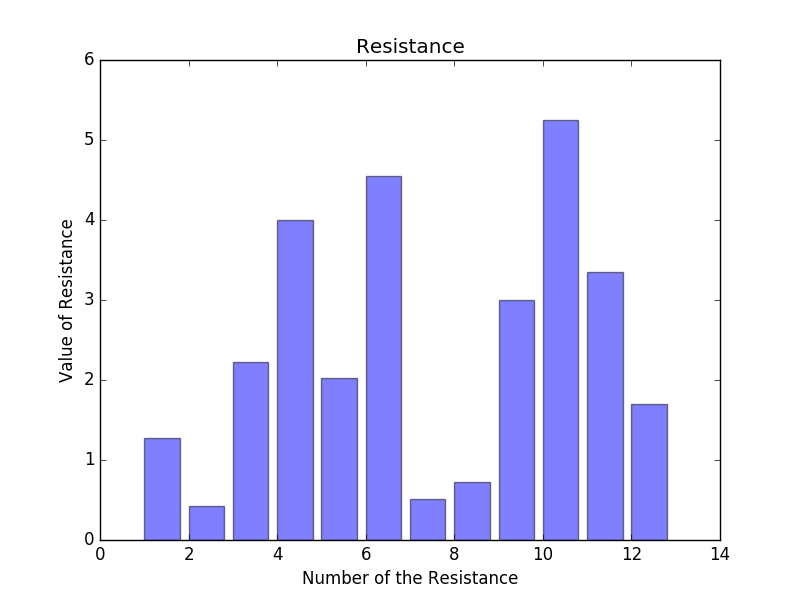
\includegraphics[width=0.4\textwidth]{img/figure2.png}
 		}
 	\end{figure}
 	저항은 $R_x = \frac{V}{5-V} R_k$로 계산되었다. 

\newpage
	
	\section{Conclusion}
	서로 다른 두 방식으로 계산된 저항을 비교해보면 대소비교에서는 일치했으나 실제 값에서는 많은 차이를 보였다.
	\begin{figure}[h]
	\centering
		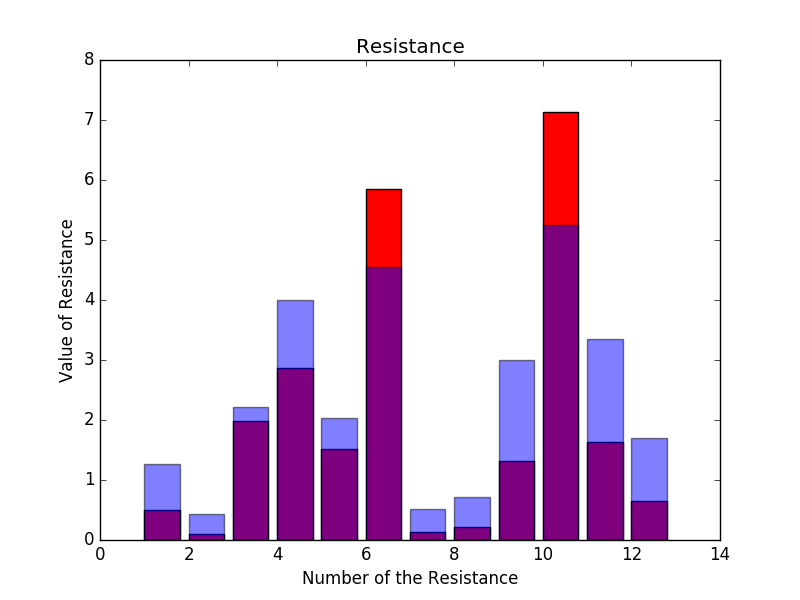
\includegraphics[width=0.4\textwidth]{img/figure3.png}
		\caption{Result의 두 그래프를 포갠 것. 빨간색이 첫 번째 그래프, 파란색은 두 번쨰 그래프, 보라색은 두 그래프가 겹친 영역을 나타낸다}
	\end{figure}

	먼저 실험에서 1,3,4,5,6을 제외하면 검류계에 흐르는 전류가 0이 되지 않았기 때문에 이것을 오차의 원인으로 볼 수 있다.
	이를 보정하기 위한 구체적인 식은 키로히호프 법칙을 통해서 유도될 수 있지만 그러면 $R_1$과 $R_2$의 비율만으로는 부족하고 각각의 값이 필요하였으나 실험에서 측정하지 못했기 때문에 본 보고서에서는 분석하지 못했다. 

	따라서 검류계의 값이 0으로 나온 1,3,4,5,6만을 이용해 두 실험의 차이를 보정해보았다.
	실험을 하면서 습동저항선의 양 끝에서 두께가 달라지는 것을 관찰할 수 있었으므로 실제 습동구리선의 길이가 20\si{cm}가 아니며 한 쪽 끝에서 가리키게까지의 거리 $l$에서 빼준 값이라고 추측하고 이를 바탕 습동구리선의 길이와 $l$을 보정하였다.
	습동 구리선이 좌우로 대칭적이라고 가정하고 양 끝의 길이가 실제로는 $a$만큼 없다고 가정하면 $R_x = \frac{20-l}{l} R_k$은 $R_x = \frac{(20-2a)-(l-a)}{(l-a)} R_k$로 볼 수 있다.
	따라서 a에 관한 다음 함수가 최소가 되는 a를 Scipy(Nelder-Mead법)를 통해서 구하였다.
	식에서 $r$는 전압계를 통해 얻은 저항값을 의미한다.
	\begin{equation}
		f(a) = \sum_{i=1}^{5} ( \frac{20-l_i-a}{l_i-a} - r ) ^2
	\end{equation}
	이를 통해 계산된 a의 값은 예상외로 -1.00238037109였다.
	이는 습동저항선이 실측값보다 짧은 것이 아니라 더 김을 뜻한다.
	습동저항선 지지대 안 쪽에 저항이 더 많이 존재하거나 습동저항선 외에 회로에서 저항을 가진 부분들에 의한 영향일 가능성도 있다. 
	다음 도표는 보정된 값을 바탕으로 계산된 두 실험의 차이를 나타낸다.
	색깔은 Figure 3의 것과 같다.
	\begin{figure}[h]
	\centering
		\subfloat[5개 실험의 원래값]{
			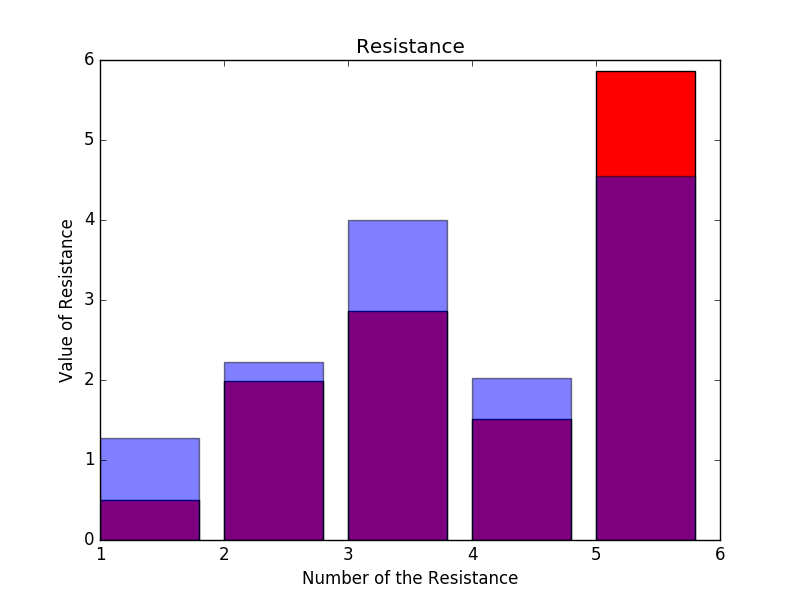
\includegraphics[width=0.4\textwidth]{img/error1.png}
		}
		\subfloat[보정된 5개의 실험값]{
			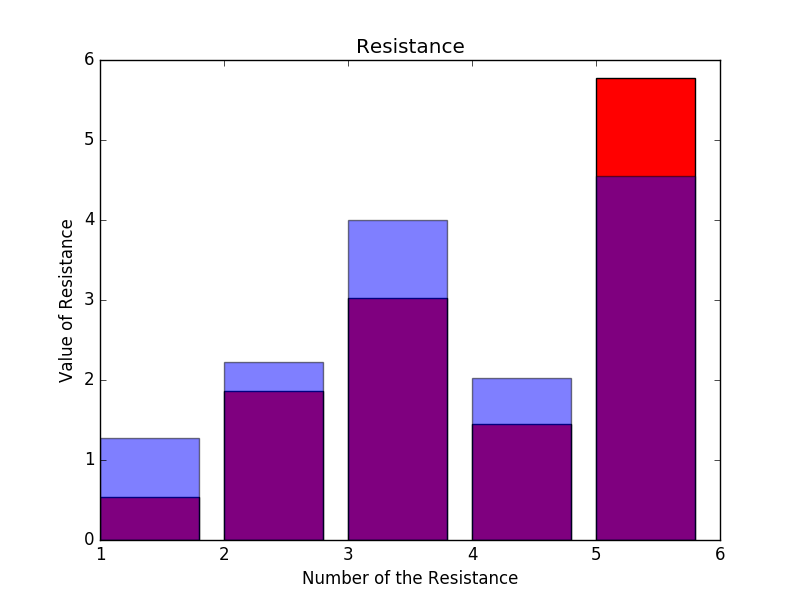
\includegraphics[width=0.4\textwidth]{img/error2.png}
		}
	\end{figure}

	그러나 이 보정만으로는 여전히 많은 오차가 남아있는 것을 볼 수 있다.
	실험 중에 있었던 현상들 중에 검류계의 값이 0에서 잘 고정되지 않고 계속해서 값이 변화한 것이 그 원인일 수 있다.
	

\section{Reference 및 부록}
	1. Halliday, D., Resnick, R., \& Walker, J. (2014). {\it{}Principles of Physics} (10th ed., Vol. 2). Hoboken, NJ: Wiley.
	\\ 

\end{document} 

%실험에서 개선할 점 등 피피티에서 봤던 거 모두 적어서 처리합시다